% TODO:
% 1) Get new SUMMARY screenshot 

\documentclass[letterpaper,12pt]{report}
\usepackage{helvet}
\usepackage[pdftex]{graphicx}

\setlength{\parindent}{0in}
\setlength{\parskip}{1.5ex plus 0.5ex minus 0.2ex}

\newlength{\sjfhmargin}
\newlength{\sjfvmargin}
\setlength{\sjfhmargin}{1in}
\setlength{\sjfvmargin}{1in}

\setlength{\voffset}{0in}
\setlength{\hoffset}{0in}

%\setlength{\headheight}{0ex}
%\setlength{\headsep}{0in}
%\setlength{\topskip}{0in}
%\setlength{\footskip}{0in}

\setlength{\textwidth}{\paperwidth}
\addtolength{\textwidth}{-2\sjfhmargin}

\setlength{\evensidemargin}{-1in}
\addtolength{\evensidemargin}{\sjfhmargin}
\setlength{\oddsidemargin}{\evensidemargin}

\setlength{\textheight}{\paperheight}
\addtolength{\textheight}{-2\sjfvmargin}
\addtolength{\textheight}{-\headheight}
\addtolength{\textheight}{-\headsep}
\addtolength{\textheight}{-\footskip}

\setlength{\topmargin}{-1in}
\addtolength{\topmargin}{\sjfvmargin}

\setlength{\parindent}{0in}
\setlength{\parskip}{1.5ex plus 0.5ex minus 0.2ex}

\usepackage[round]{natbib}

\ifx\pdfoutput\undefined \newcount\pdfoutput \fi
\ifcase\pdfoutput
  \special{papersize=11in,8.5in}
\else
  %\usepackage{thumbpdf}
  \usepackage[pdftex]{hyperref}
  \pdfpagewidth 8.5truein
  \pdfpageheight 11truein
  \pdfhorigin 1truein
  \pdfvorigin 1truein
  \hypersetup{
    pdfstartpage=1,
    pdftitle={VERITAS Positioner Control Software},
    pdfsubject={VERITAS Positioner Control Software Manual},
    pdfkeywords={VERITAS,software,tracking},
    pdfauthor={\textcopyright\ Stephen Fegan},
    pdfcreator={\LaTeX\ with package \flqq hyperref\frqq}
  }
  \pdfinfo{/CreationDate (D:20040420200000)}
\fi

\usepackage{fancyhdr}
\pagestyle{fancy}
\fancyhead{}
\fancyhead[L]{\bfseries VERITAS Positioner Control Software Manual}
\fancyhead[R]{\bfseries Version 1.1.0}
\fancyfoot[C]{\bfseries UCLA}
\fancyfoot[L]{\bfseries Stephen Fegan}
\fancyfoot[R]{\bfseries \thepage}
\renewcommand{\headrulewidth}{0.4pt}
\renewcommand{\footrulewidth}{0.4pt}

\renewcommand{\baselinestretch}{1.5}

\def\two@digits#1{\ifnum#1<10 0\fi\number#1}
\edef\today{\the\year-\two@digits{\the\month}-\two@digits{\the\day}}

\begin{document}
\thispagestyle{empty}
\title{VERITAS Positioner Control Software Manual}
\author{Stephen Fegan \\ University of California, Los Angeles \\ \texttt{sfegan@astro.ucla.edu} }
%\date{2004-04-16}
\maketitle

\thispagestyle{empty}
\vspace*{\fill}
\centerline{\setlength{\fboxrule}{3pt}\setlength{\fboxsep}{.2in}
\fbox{\large\begin{minipage}{0.9\textwidth}
{\bfseries\Huge CAUTION}\\[2ex] The positioner/OSS combination is a
large and powerful machine. If used improperly, it can damage itself,
damage vehicles, damage structures and injure or kill people. This
manual documents only the Ethernet \& Serial Control Program. It is
not a manual on the operation of the telescope positioner or the steps
required for its safe use. Ensure that you have read and that you
understand the \textit{VERITAS Positioner Operations} manual before
attempting to operate the positioner. Familiarize yourself with the
saftey interlock system and do not attempt to override the interlock
sensors without supervision from FLWO staff. Never operate the
positioner when people are working on the structure or while the
system is locked out and/or tagged out. Finally, never leave the
positioner unattended while it is being operated.
\end{minipage}}}
\vspace*{\fill}

\chapter*{Abstract}
\thispagestyle{fancy}
\setcounter{page}{1}

This document describes the use of the VERITAS Ethernet and Serial
Telescope Control program. The program provides control over the RPM
positioner using either the Ethernet or RS422 (serial line) based
command protocols. The program can be used to track sources while
making routine observations and as a backup to the primary VERITAS
control program in the case of failure of the Ethernet based control
hardware. The normal operation of the program is described in
chapter~\ref{CHAP::NORMAL}. This chapter descibes the three primary
information screens of the program in which movement commands can be
entered and targets chosen for tracking. 
Chapter~\ref{CHAP::CORRECTIONS} describes the corrections model used
to track targets accurately, how to change the parameters of the model
manually and how to take pointing measurements and automatically
optimize the model. Use as a failsafe control system is described in
chapter~\ref{CHAP::FAILSAFE}. Finally, in chapter~\ref{CHAP::CODE},
the layout of the program code is described along with the in-built
emulator which can be used to test changes to the code.

\chapter{Theory of Operation}
\label{CHAP::NORMAL}
\thispagestyle{fancy}

The positioner control system (PCS) comprises a complex set of
interconnected components whose purpose is to allow the telescope
track celestial objects accurately, and to ensure the integrity of the
positioner, drive system, optical support structure and all components
attached to the telescope such as the mirrors and focus box. This
chapter briefly outlines the various components within the PCS and
describes how they contribute to achieving these requirements.

\section{Overview of the PCS}

As with many modern control systems, the PCS consists of a number of
interacting components. At one end of the control system is the servo
amplifier which provides current to the motors driving each axis and
the encoders and tacometers which provide feedback of the mount
position and speed. At the other end of the control chain is the
tracking software which is responsible for communicating the
operator's commands to the positioner, for monitoring and displaying
the positioner status and for proving timely updates of the target
position to the positioner if it is commanded to track a celestial
object.

These two ends of the control chain are joined by a number of hardware
and software components inside the positioner. Understanding how these
components interact will help in diagnosing problems that may occur
during operation, such as loss of connection to the positioner.
Figure~\ref{FIG::PCS} shows the components of the PCS and how commands
and data flow between them.

\begin{figure}
\centerline{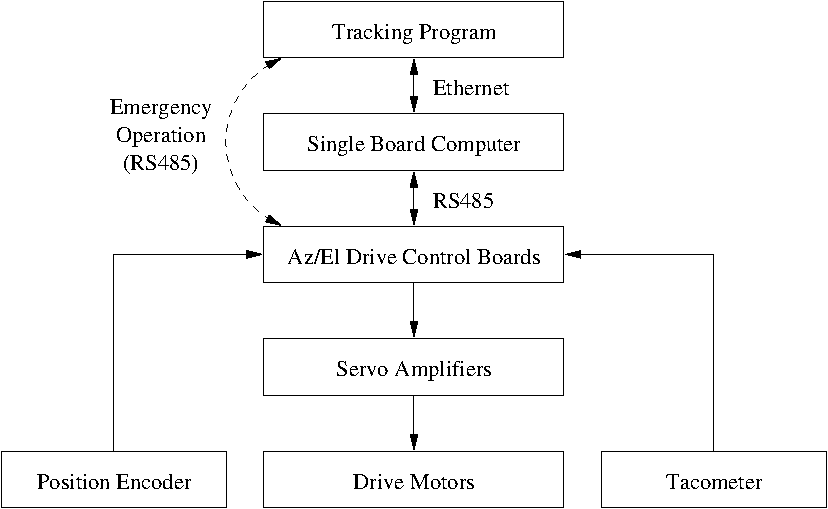
\includegraphics[width=0.8\textwidth]{graphics/pcs_components.pdf}}
\caption{\label{FIG::PCS}PCS component flowchart}
\end{figure}

During normal operation the tracking program communicates with a based
single board computer (SBC)\footnote{Microsys model SBC1490 --
Advanced 486DX PC/104 Embedded PC} in the positioner over
Ethernet. The SBC is connected to the tracking control boards over a
serial connection using RS422. When power is applied the SBC boots up
DOS and starts running software supplied by RPM. The software listens
for UDP datagrams from the tracking software, which are received over
Ethernet. When a datagram is received, the software decodes the
command, extracting any parameters that sent. It then issues commands
to the tracking control boards using the serial protocol that these
boards understand. Any command parameters are encoded as required by
this protocol. Some UDP protocol commands require multiple serial
protocol commands to be executed. If the particular command requires
the return of data then the responses made by the tracking control
boards are decoded and re-encoded for transmission back to the
tracking control software in a UDP datagram. If the particular command
does not return data than an acknowledgment datagram is sent. In
essence, the SBC acts as a protocol translater, i.e. it does nothing
more than translate between the UDP based protocol and the RS422 based
protocol.



\section{UDP Protocol}

\section{RS422 Protocol}

\chapter{Normal operation}
\label{CHAP::NORMAL}
\thispagestyle{fancy}

During routine operation, the telescope is controlled from the
graphical user interface (GUI) of tracking program. The GUI allows the
telescope operator to perform all of the functions required during
normal operation, such as to slew the telescope, conveniently select
and track sources and stop the telescope motion. It provides regular
updates of the positioner status and indicates if any error condition
occurs.

Behind the scenes, the tracking program constantly communicates with
the positioner. Every 250\,ms the program reads the status of the
positioner and commands it to either remain stationary, slow down,
slew or track a target as appropriate. It applies a simple model
accounting for misalignments and flexure in the telscope to convert
the location of the target in the sky into values of azimuth and
elevation drive angles. These ``tracking correction'' parameters are
are described in Chapter~\ref{CHAP::CORRECTIONS}.

The tracking program was constructed with the assumption that has
exclusive control of the telescope. If another instance of the program
is running or if the telescope control unit (TCU) supplied by RPM is
actively sending commands to the mount then conflicts will occur. For
example the positioner may be instructed to slew and to apply the
brake at the same time, which will lead to unpredictable behaviour. 
Therefore it is important to run only one instance of the program at
any time.  Conversely, if the positioner does not seem to be
responding the operator should first ensure that no other instance of
the program is running.

\section{Starting tracking operations}

Under normal conditions commencing tracking operation with the first
VERITAS telescope is simply a matter of:
\begin{enumerate}
\item checking that it is safe to do so,
\item turning on power to the positioner and
\item starting the tracking program.
\end{enumerate}

Before moving the telscope for the first time each night check that it
is safe to do so. Firstly, ensure that nobody is working on the
telescope Walk around the instrument making sure that any equipment
that was used during the day is moved to a safe distance. In
particular ensure that the man lifts are far enough from the OSS that
they cannot be hit by the instrument when it slews. Check that all
access hatches are securely closed. Finally, on the panel beside the
lower access hatch check that the hand-paddle controller is not
plugged in (see Section~XXX) and place the RUN/SAFE interlock switch
into the SAFE position.

Turn the power to the mount on. The mount power is switched off at the
end of each night at the breaker box between the trailer and the
UPS/Laser shed. The breaker box is mounted upright and covered with a
sheet metal lid which is opened by lifting from the bottom. The
appropriate breaker is a large three-phase switch marked
``Positioner''. Switch the breaker on making sure not to hit off the
others -- breakers are spring loaded, a light touch is sufficient to
make them trip.

Before starting the tracking program switch off the Telescope Control
Unit (TCU -- see Figure~XXX). At time of writing, the tracking program
for the first VERITAS telescope is installed on the array control
computer in the trailer. Ensure that there is not already a copy of
the program running -- check all the desktops on the
array control computer.

The tracking program can be started from a x-windows terminal by
typing:
\begin{verbatim}
cd /home/observer/steering
./serial_tracking
\end{verbatim}
The tracking program occasionally prints messages to the terminal from
which it was started, so it is preferable to run the program in the
foreground and reserve the x-windows terminal exclusively for any
messages that are printed. Then, if any error conditions arise or the
program crashes for some reason the debugging messages will be easily
accessable.

After a few moments the tracking GUI should appear and the program
attempts to connect with the positioner over Ethernet. Assuming that a
connection is made the GUI looks similar to
Figure~\ref{FIG::GUI_CONNECETION}. If a connection to the
mount cannot be made the display looks similar to
Figure~\ref{FIG::GUI_NOCONNECTION}, see
Chapter~\ref{CHAP::TROUBLESHOOTING} for trouble shooting suggestions.

\begin{figure}[p]
\centerline{\framebox{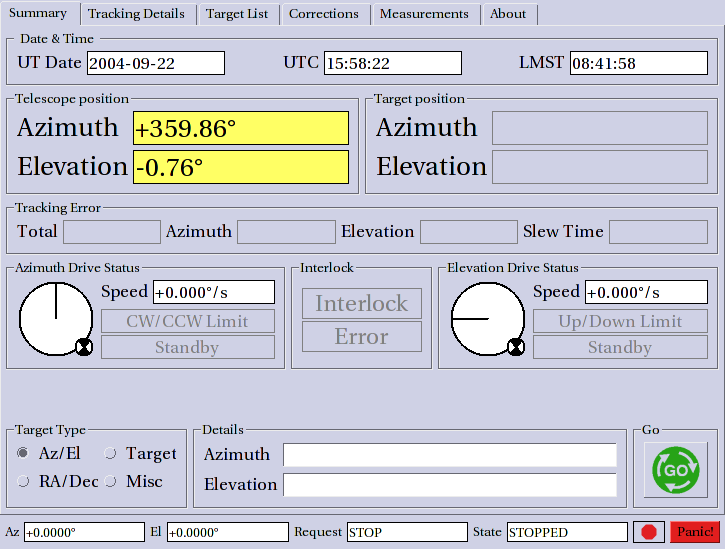
\includegraphics[width=0.66\textwidth]{graphics/screen_summary_connection.png}}}
\caption{\label{FIG::GUI_CONNECTION} Graphical user 
interface when successful connection is made to the positioner.}
\end{figure}

\begin{figure}[p]
\centerline{\framebox{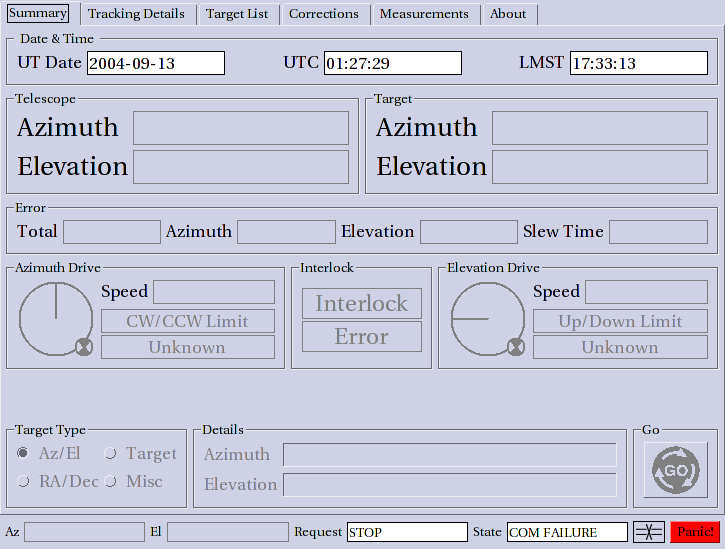
\includegraphics[width=0.66\textwidth]{graphics/screen_summary_noconnection.png}}}
\caption{\label{FIG::GUI_NOCONNECTION} Graphical user 
interface when a connection cannot be made to the positioner.}
\end{figure}

\section{Graphical user interface}

The GUI is organised into a number of pages which are selected through
``tabs'' at the top of the interface. Initially the tracking summary
page is visible; this fact is indicated by the \textbf{Summary} tab at
the top of the interface which appears to be raised higher the other
tabs. 

The \textbf{Summary} page displays the minimal information required to
monitor the operation of the instrument. It also provides controls
which allow the operator to select targets and start/stop
tracking. The other pages, which provide various other positioner
information and control functionality, can be selected by clicking on
the appropriate tab.  For example, the \textbf{Tracking Details} tab
displays all of the information which is gathered from the positioner
and the \textbf{Target List} provides a convenient list of all loaded
targets and allows them to be selected for tracking. These first three
pages are descibed in detail in the remainder of this chapter.  The
next two, labelled \textbf{Corrections} and \textbf{Measurements} are
described in detail in Chapter~\ref{CHAP::CORRECTIONS}. Finally, the
\textbf{About} page shows information about the tracking program and
will not be commented on further.

\subsection{Status bar}

The status bar, displayed along the bottom of the interface, provides
information about the current status of the positioner. This
information is visible no matter what page is selected in main part of
the GUI. The information supplied in this area allows the operator to
monitor the tracking while performing other actions, such as using the
\textbf{Target List} page to select the next target to track. The
following items are displayed:

\subsubsection{Az and El} 

Azimuth and elevation drive angles reported by the positioner. No
tracking corrections are applied to these values.

\subsubsection{Request}

The tracking state requested by the operator:
\begin{itemize}
\item \textbf{STOP}: the program has been requested to bring the 
positioner safely to a halt and apply the brakes once it is
stopped.
\item \textbf{SLEW}: the program has been requested to 
slew the positioner to a target and switch to \textbf{STOP} mode once it
has been reached.
\item \textbf{TRACK}: the program has been requested to
slew the positioner to a target and track it thereafter.
\end{itemize}

\subsubsection{State}

The actual state of tracking, which may be
different from the requested state:
\begin{itemize}
\item \textbf{STOPPED}: the telscope is stopped and brakes are applied.

\item \textbf{SLEWING}: the telescope is slewing to a target location.

\item \textbf{TRACKING}: the telescope is tracking a target. 

\item \textbf{SLEWING TO KEY}: the telescope is either moving
into or out of the key. The telescope must move to elevation greater
than 15$^\circ$ before it can move substantially in
azimuth. Similarly, to move to elevation less than 15$^\circ$ (i.e. to
return to the home position), it must first move to within a few
degrees of zero azimuth.

\item \textbf{RAMPING DOWN}: following a request to \textbf{STOP}, 
the telescope is slowing a safe rate of deceleration before applying
the brakes.

\item \textbf{COM FAILURE}: communication with the positioner has been 
lost.
\end{itemize}

\subsubsection{Motion/status indicator icon}
Second to last is the motion and status indicator. It provides the
operator with an immediate visual cue as to the status of the
instrument. When the state is
\textbf{STOPPED}, it appears as a rad, octagonal stop sign 
(Figure~\ref{FIG::GUI_CONNECTION}). When
\textbf{SLEWING}, \textbf{TRACKING}, \textbf{SLEWING TO KEY}, or
\textbf{RAMPING DOWN}, its appearance is of an animated, rotating, broken 
circle on a greeen background (Figure~\ref{FIG::GUI_SUMMARY}), whose speed
depicts the speed at which the instrument is moving. When
communication to the positioner is lost, i.e. the state is
\textbf{COM FAILURE}, the indicator appears as a set of wires with
a break in them with animated messages getting stopped at the break,
Figure~\ref{FIG::GUI_NOCONNECTION}.

\subsubsection{PANIC}

Panic button, pushing this button commands the positionor to
immediatly apply the brakes, then exits the program. This command is
not issued through the telescope controller thread in the program and
will may therefore be useful if the controller thread is not
responding. To draw attention to this important button, it slowly
oscillates in color between two different shades of red... this is its
normal behavior an should not cause the operator to panic!

\subsection{Summary Page}

The summary page presents the most relevant infomation required to
monitor the status of the telescope tracking. The following
information and controls are present:

\begin{figure}
\centerline{\framebox{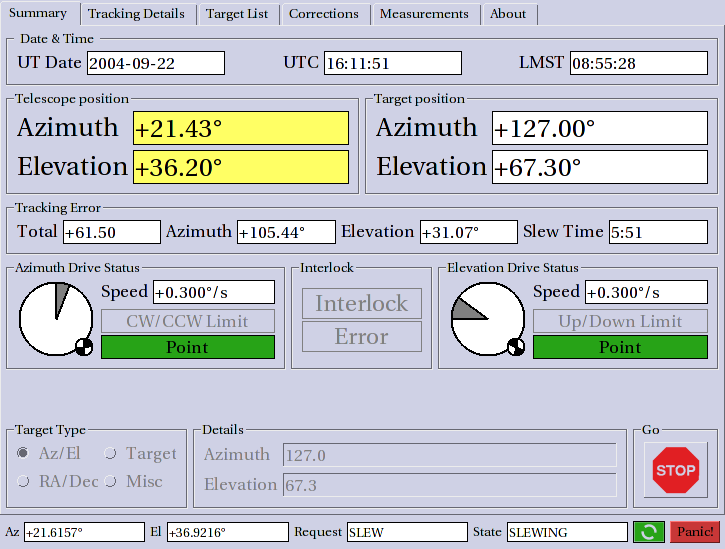
\includegraphics[width=0.66\textwidth]{graphics/screen_summary.png}}}
\caption{\label{FIG::GUI_SUMMARY} Summary page while slewing to a selected
target azimuth and elevation.}
\end{figure}

\subsubsection{Time \& Date}
The data and time, as provided by the operating system, in coordinated
universal time (UTC). Before operating the telescope, the time should
be checked against a GPS clock to ensure that it is correct. If it is
not, see Section~XXX. The local mean sidearal time (LMST) is also
shown in this panel.

\subsubsection{Telescope Position}

The current azimuth and elevation of the telescope after the (inverse)
tracking correction model had been applied. This position therefore
corresponds to the direction of the optic axis in the sky. The values
displayed here should not, in general, agree with the raw drive angle
values displayed at the bottom of the program, which do not have the
correction model applied. Since it is important to see where the
telescope is pointing at a glance, the \textbf{Telescope Position} are
displayed against a yellow background.

\subsubsection{Target Position}

The current azimuth and elevation of the target in the sky. If no
target is selected, these values are not displayed. When tracking an
object, the target and telescope positions should be roughly the same.
The background color of the aziumuth and elevation position display
provided information about the target:
\begin{itemize}
\item \textbf{AZ\&EL Solid White}: target can be tracked by the
telescope

\item \textbf{AZ\&EL Solid Red}: target is outside of allowed range
of motion of positioner: either with elevation below 15$^\circ$,
outside of the key or too high, with drive angle $>90^\circ$, which
can occur with some tracking correction settings.

\item \textbf{AZ\&EL Solid Yellow}: the target will be outside the
allowed range of motion (see above) within the next 30 minutes. This
serves as a warning against starting a run on the target.

\item \textbf{AZ Flashing Red}: the target is moving faster than the
maximum allowed azimuth speed and therefore cannot be tracked
accurately at this time. This occurs occasionally for sources which
transit very close to the zenith. Tracking does not stop when this
occurs, the instrument just falls behind the target.

\item \textbf{AZ Flashing Yellow}: the target will move faster than the
maximum allowed azimuth speed over the next 30 minutes. See above.
\end{itemize}

\subsubsection{Tracking Error}

\textbf{Total}, the angular distance between the current telescope position
and the target position, in degrees. \textbf{Azimuth}, the distance in
azimuth between to the target. \textbf{Elevation}, the distance in
elevation between to the target. \textbf{Slew Time}, indicates the time 
in (MM:SS) required to slew at maximum speed to the target location.

\subsubsection{Azimuth Drive Status}


\subsubsection{Interlock}

\subsubsection{Elevation Drive Status}

\subsubsection{Target Type}

\subsubsection{Details}

\subsubsection{Go}


\chapter{Tracking corrections}
\label{CHAP::CORRECTIONS}
\thispagestyle{fancy}

\chapter{Failsafe operation}
\label{CHAP::FAILSAFE}
\thispagestyle{fancy}

\chapter{Code description}
\label{CHAP::CODE}
\thispagestyle{fancy}

\chapter{Troubleshooting}
\label{CHAP::TROUBLESHOOTING}
\thispagestyle{fancy}

Multiple instances

Power

\chapter{Motion Control System}
\label{CHAP::MCS}
\thispagestyle{fancy}

The VERITAS telescopes use a sophisticated motion control system (MCS)
to provide smooth tracking and to ensure the integretry of the
positioner. Schematically, the MCS consists of the following elements

\begin{itemize}
\item Tracking control software
\item Ethernet interface
\item Trajectory generators
\item Position loops -- PID/Vff filter
\item Velocity loops -- PI filter
\item Pedestal inteface
\item Dual-drive controller
\item Servo amplifiers
\item Servo motors
\item Sensors (Limit switches, encoders and tachometer)
\end{itemize}

Most of these items function transparently to the operator and require
no tuning. In fact, unless there is a failure, the only components
that need adustment are the positioner and velocity PIDs and
trajectory generators.

\section{Position loop -- PID/Vff filter}

The most visible component of the MCS is the digital position loop
which consists of a PID (Proportional, Integral, Derivative) motion
filter with Velocity Feed-Forward (VFF). A PID is a feedback system
whose output depends on the difference between the target (commanded)
position and the measured (actual) position. The output from the PID
ultimately controls the amount of current in the motors, hence the
torque applied to the telescope and its slewing velocity. The output
from the PID part of the filter is the sum of three components:

\begin{itemize}
\item The first component is proportional to the directly positional
error, resulting in a large torque and velocity when the telescope is
far from the commanded position. In general the positioner will
accelerate as a result of the motor currenr, causing the it to move to
the commanded position. As it closes in the proportional term
decreases and hence so does the velocity, until (ideally) the
telescope settles at its commanded position. The size of the
proportional contribution to the PID output is determined by the
\textbf{proportional gain}, $K_P$.

\item The second component is proportional to the total error accumated
over some number of recent loop iterations. This ``integral''
component quantifies whether the measured position is systematically
behind or ahead of the target position. If this is the case, the
integral component will grow, contributing more to the PID output, and
forcing the system to catch up with the target position (or slow down
if the telescope leads the target). The degree to which the output of
the PID depends on this integrated error is determined by the 
\textbf{integral gain}, $K_I$. Integral gain is generally essential
to eliminate (or at leat minimize) steady state tracking
errors. However, a large integral gain tends to cause overshoot and
oscillations. If the system is constantly behind the target, for
example while slewing, the integral component can become quite large,
and will tend to keep the positioner moving even though the target
position has been reached, and even passed. This effect, called
integral wind-up, occurs because a large inegral component can only be
eliminated by having the error change sign and be integrated for some
number of cycles, until the integral componet is eliminated. In many
PID systems this effect is minimized by limiting the integral in some
manner. A number of schemes are possible, in the VERITAS MCS the
integral is only taken over a finite number of previous samples,
determined by the \textbf{integration limit} parameter.

\item The final component of the PID filter is proportional to the
instantaneous rate of change of the positional error. When the error
is constant over time, the differential term is zero. If the error is
increasing the term acts to promote motion of the telescope towards
the target; if the error is decreasing the differential term acts to
slow and stop the motion. The size of the derivative contribution to
the PID output is determined by the \textbf{derivative gain}, $K_D$.
\end{itemize}

The final contribution to the output of the MCS comes from velocity
feed-forward, which is not a traditional PID term. It is easy to see
that with only P, I and D terms the system \textbf{cannot} follow a
moving target without an (albeit possibly small) error. For example,
if the target is moving at a relatively constant rate and the
positioner is following steadily, then the derivative term is zero (as
the error is constant). If $K_I=0$ the current to drive the motor,
which must come through a non-zero PID output, can only be generated
by the proportional term from a non-zero positional error. If $K_I \ne
0$ then the integral term also contributes and the positional error
required to generate the motor current is smaller, but must still be
present.

VFF is proportional to the instantaneous target velocity. The size of
the component is determined by the $K_{vff}$ gain. Unlike the
traditional PID terms, VFF does not have any feedback, in the sense
that it does not depend on the telescope position (or positional
error). In an ideal system, all of the current required to drive the
motors while tracking a moving source would come from velocity
feed-forward, and the PID would provide additional current to slew to
the source and to elimate any drift from the target position.

If the target position at time slice $i$ is $P_T(t_i)$ and the
measured position is $P_M(t_i)$ then the error, $E(t_i)$, and output
of the MCS, $O(t_i)$, are \footnote{The exact relation of the PID
output to its inputs and gains depends on the specific motion control
chip in the MCS. This is valid for ACS-Tech80 model 594x, which, I
believe, were used by RPM.},

$\displaystyle E(t_i) = P_T(t_i)-P_M(t_i)$ and

$\displaystyle O(t_i) = 
K_P\,E(t_i) + 
K_D\,\left[E(t_i)-E(t_{i-1})\right] +
\frac{K_I}{256} \sum_{j=0}^{ILim}E(t_{i-j}) +
\frac{K_{Vff}}{4}\left[P_T(t_i)-P_T(t_{i-1})\right]$.

-- noise - size of gains 

-- advice for tuning

-- reference to MCS documentation

\section{Trajectory generator}

The gains in the PID/VFF loop must be chosen to give good performance
while tracking slowly moving astronomical targets. For example, if the
target is moving at $0.005^\circ/s$ and the telescope is required to
track to within $0.001^\circ$ with a PID system tuned to have only a
proportional component, then the PID output of $0.001 K_P$ must result
in a velocity of $0.005^\circ/s$. If the system is now asked to slew a
large distance, say $40^\circ$ and there is a linear relationship
between the PID/VFF and velocity, then a velocity of $200^\circ/s$
results. In practical terms this would result in a PID output voltage
that is saturated against the supply rail and an unregulated (unsafe)
motion\footnote{Analogous to driving a car by either having your foot
hard on the accelerator and hard on the brakes.}. It is therefore
desirable to supply a target position to the PID which results in an
error that has the same magnitude as that present while tracking.

This is achieved by a trajectory generator (also known as a set-point
scheduler). When the MCS is commanded by the tracking software to slew
to a target, the trajectory generator plans a smooth path from the
current location to the target position. The VERITAS MCS uses a
trapezoidal velocity profile, consisting of three phases:
acceleration, constant velocity and deceleration, to arrive at the
commanded position. The motion profile is parameterized by two
parameters, the \textbf{maximum velocity} ($v_{max}$) and
\textbf{acceleration} ($a_{max}$).

The trajectory generator runs inside the position loop, and sets the
target position of the PID/VFF to the next point along the path each
iteration. The profile generator does not have any feedback from the
actual telescope motion. When a slew command is received, a profile is
produced and the PID is expected to make the telescope follow that
profile. If it fails to do so, and the telescope falls behind (or in
the extreme case, oscillates wildly), the profile is not adjusted to
compensate. Therefore, if the PID is badly tuned then the $v_{max}$
and $a_{max}$ parameters do not, necessarily, correspond to the
maximum velocity and acceleration with which the telescope moves.
For example, if large oscillations are present then the acceleration
at the peaks of the oscillation can be considerably larger than the
requested maximum as can the peak velocity between the peaks. In one
such case seen with T2 during commissioning of the servo system, a
requested maximum velocity of $0.3^\circ/s$ resulted in oscillatory
motion with a maximum speed of $0.6^\circ/s$.

-- some figures might be nice

-- tuning

\section{Velocity Loop -- PI filter}


\section{Pedestal inteface}


\section{Dual Drive Controller}


\section{Servo Amplifier}


\end{document}
